\documentclass[a4paper]{article}

\input{style/ch_xelatex.tex}
\input{style/scala.tex}

%代码段设置
\lstset{numbers=left,
basicstyle=\tiny,
numberstyle=\tiny,
keywordstyle=\color{blue!70},
commentstyle=\color{red!50!green!50!blue!50},
frame=single, rulesepcolor=\color{red!20!green!20!blue!20},
escapeinside=``
}

\graphicspath{ {images/} }
\usepackage{ctex}
\usepackage{graphicx}
\usepackage{color,framed}%文本框
\usepackage{listings}
\usepackage{caption}
\usepackage{amssymb}
\usepackage{enumerate}
\usepackage{xcolor}
\usepackage{bm}
\usepackage{lastpage}%获得总页数
\usepackage{fancyhdr}
\usepackage{tabularx}
\usepackage{geometry}
\usepackage{minted}
\usepackage{graphics}
\usepackage{subfigure}
\usepackage{float}
\usepackage{pdfpages}
\usepackage{pgfplots}
\pgfplotsset{width=10cm,compat=1.9}
\usepackage{multirow}
\usepackage{footnote}
\usepackage{booktabs}

%-----------------------伪代码------------------
\usepackage{algorithm}
\usepackage{algorithmicx}
\usepackage{algpseudocode}
\floatname{algorithm}{Algorithm}
\renewcommand{\algorithmicrequire}{\textbf{Input:}}
\renewcommand{\algorithmicensure}{\textbf{Output:}}
\usepackage{lipsum}
\makeatletter
\newenvironment{breakablealgorithm}
  {% \begin{breakablealgorithm}
  \begin{center}
     \refstepcounter{algorithm}% New algorithm
     \hrule height.8pt depth0pt \kern2pt% \@fs@pre for \@fs@ruled
     \renewcommand{\caption}[2][\relax]{% Make a new \caption
      {\raggedright\textbf{\ALG@name~\thealgorithm} ##2\par}%
      \ifx\relax##1\relax % #1 is \relax
         \addcontentsline{loa}{algorithm}{\protect\numberline{\thealgorithm}##2}%
      \else % #1 is not \relax
         \addcontentsline{loa}{algorithm}{\protect\numberline{\thealgorithm}##1}%
      \fi
      \kern2pt\hrule\kern2pt
     }
  }{% \end{breakablealgorithm}
     \kern2pt\hrule\relax% \@fs@post for \@fs@ruled
  \end{center}
  }
\makeatother
%------------------------代码-------------------
\usepackage{xcolor}
\usepackage{listings}
\lstset{
breaklines,%自动换行
basicstyle=\small,
escapeinside=``,
keywordstyle=\color{ blue!70} \bfseries,
commentstyle=\color{red!50!green!50!blue!50},%
stringstyle=\ttfamily,%
extendedchars=false,%
linewidth=\textwidth,%
numbers=left,%
numberstyle=\tiny \color{blue!50},%
frame=trbl%
rulesepcolor= \color{ red!20!green!20!blue!20}
}

%-------------------------页面边距--------------
\geometry{a4paper,left=2.3cm,right=2.3cm,top=2.7cm,bottom=2.7cm}
%-------------------------页眉页脚--------------
\usepackage{fancyhdr}
\pagestyle{fancy}
\lhead{\kaishu \leftmark}
% \chead{}
\rhead{\kaishu 深度学习进阶课 实验报告}%加粗\bfseries
\lfoot{}
\cfoot{\thepage}
\rfoot{}
\renewcommand{\headrulewidth}{0.1pt}
\renewcommand{\footrulewidth}{0pt}%去掉横线
\newcommand{\HRule}{\rule{\linewidth}{0.5mm}}%标题横线
\newcommand{\HRulegrossa}{\rule{\linewidth}{1.2mm}}
\setlength{\textfloatsep}{10mm}%设置图片的前后间距
%--------------------文档内容--------------------

\begin{document}
\renewcommand{\contentsname}{目\ 录}
\renewcommand{\appendixname}{附录}
\renewcommand{\appendixpagename}{附录}
\renewcommand{\refname}{参考文献}
\renewcommand{\figurename}{图}
\renewcommand{\tablename}{表}
\renewcommand{\today}{\number\year 年 \number\month 月 \number\day 日}

%-------------------------封面----------------
\begin{titlepage}
    \begin{center}
    \includegraphics[width=0.8\textwidth]{NKU.png}\\[1cm]
    \vspace{20mm}
		\textbf{\huge\textbf{\kaishu{计算机学院}}}\\[0.5cm]
		\textbf{\huge{\kaishu{语音信息处理实验报告}}}\\[2.3cm]
		\textbf{\Huge\textbf{\kaishu{基于 ECAPA-TDNN 的说话人识别：\\[0.3cm]嵌入空间、鲁棒性与 ASV/ASI}}}

		\vspace{\fill}

    % \textbf{\Large \textbf{并行程序设计期末实验报告}}\\[0.8cm]
    % \HRule \\[0.9cm]
    % \HRule \\[2.0cm]
    \centering
    \textsc{\LARGE \kaishu{姓名\ :\ 申健强}}\\[0.5cm]
    \textsc{\LARGE \kaishu{学号\ :\ 2313119}}\\[0.5cm]
    \textsc{\LARGE \kaishu{专业\ :\ 计算机科学与技术}}\\[0.5cm]

    \vfill
    {\Large \today}
    \end{center}
\end{titlepage}

\renewcommand {\thefigure}{\thesection{}.\arabic{figure}}%图片按章标号
\renewcommand{\figurename}{图}
\renewcommand{\contentsname}{目录}
\cfoot{\thepage\ of \pageref{LastPage}}%当前页 of 总页数


% 生成目录
\clearpage
\tableofcontents
\newpage

%--------------------------正文--------------------------------
\section{实验目的与内容}
本实验使用在中文数据集 CN-Celeb 上预训练的 SpeechBrain 说话人嵌入模型 ECAPA-TDNN
（\texttt{LanceaKing/spkrec-ecapa-cnceleb}），不做重新训练，在一个小规模 AISHELL 子集
（\texttt{aishell\_mini}）上完成从嵌入提取、空间分析到下游识别的完整流程。实验分为三部分：

\begin{enumerate}
  \item 课程一（15\%）：配置 SpeechBrain 环境，加载预训练 ECAPA-TDNN，读取示例音频提取 192 维说话人嵌入，
        理解 checkpoint 的模块构成与 \texttt{encode\_batch} 流程。
  \item 课程二（35\%）：批量提取干净语音的嵌入并用 t-SNE 可视化，再对同一批语音施加加噪、8k 电话信道与变调
        三种扰动，用嵌入漂移衡量模型鲁棒性。
  \item 课程三（50\%）：基于嵌入构建说话人模板，实现说话人验证（ASV）与说话人辨认（ASI）。
        在 dev 集上确定等错误率 EER 对应的阈值 $\tau^\ast$，在 test 集上评测，并完成闭集与开集辨认；
        加分项在冻结嵌入上训练一个线性分类头。
\end{enumerate}

实验环境为 speechbrain conda 环境（Python 3.10.20，torch 2.1.2+cu118，torchaudio 2.1.2+cu118，
speechbrain 1.1.0），推理运行于 GPU（NVIDIA RTX 4060 Laptop）。SpeechBrain 1.1.0 调用了
\texttt{torch.amp.custom\_fwd(device\_type=...)}，torch 2.1.2 尚无该签名，因此加载模型前先安装一个 shim
把它转发到 \texttt{torch.cuda.amp}，保证前向计算正常。

\section{实验原理}
说话人识别的核心是把任意长度的语音映射成一个固定维度的向量，即说话人嵌入，使同一说话人的语音嵌入彼此接近、
不同说话人的相互远离，从而把识别问题变成向量之间的相似度比较。本实验采用的 ECAPA-TDNN\cite{ecapa}
在 x-vector 的基础上引入 SE-Res2Net 多尺度模块、多层特征聚合和通道注意力统计池化，
把变长的帧级特征压缩为句子级的 192 维嵌入（图~\ref{fig:ecapa}）。模型训练时在嵌入上接一个分类头，
用角度间隔损失（AAM-Softmax）在角度空间上区分说话人；推理时丢弃分类头，只用嵌入网络做通用特征提取器。

\begin{figure}[H]
    \centering
    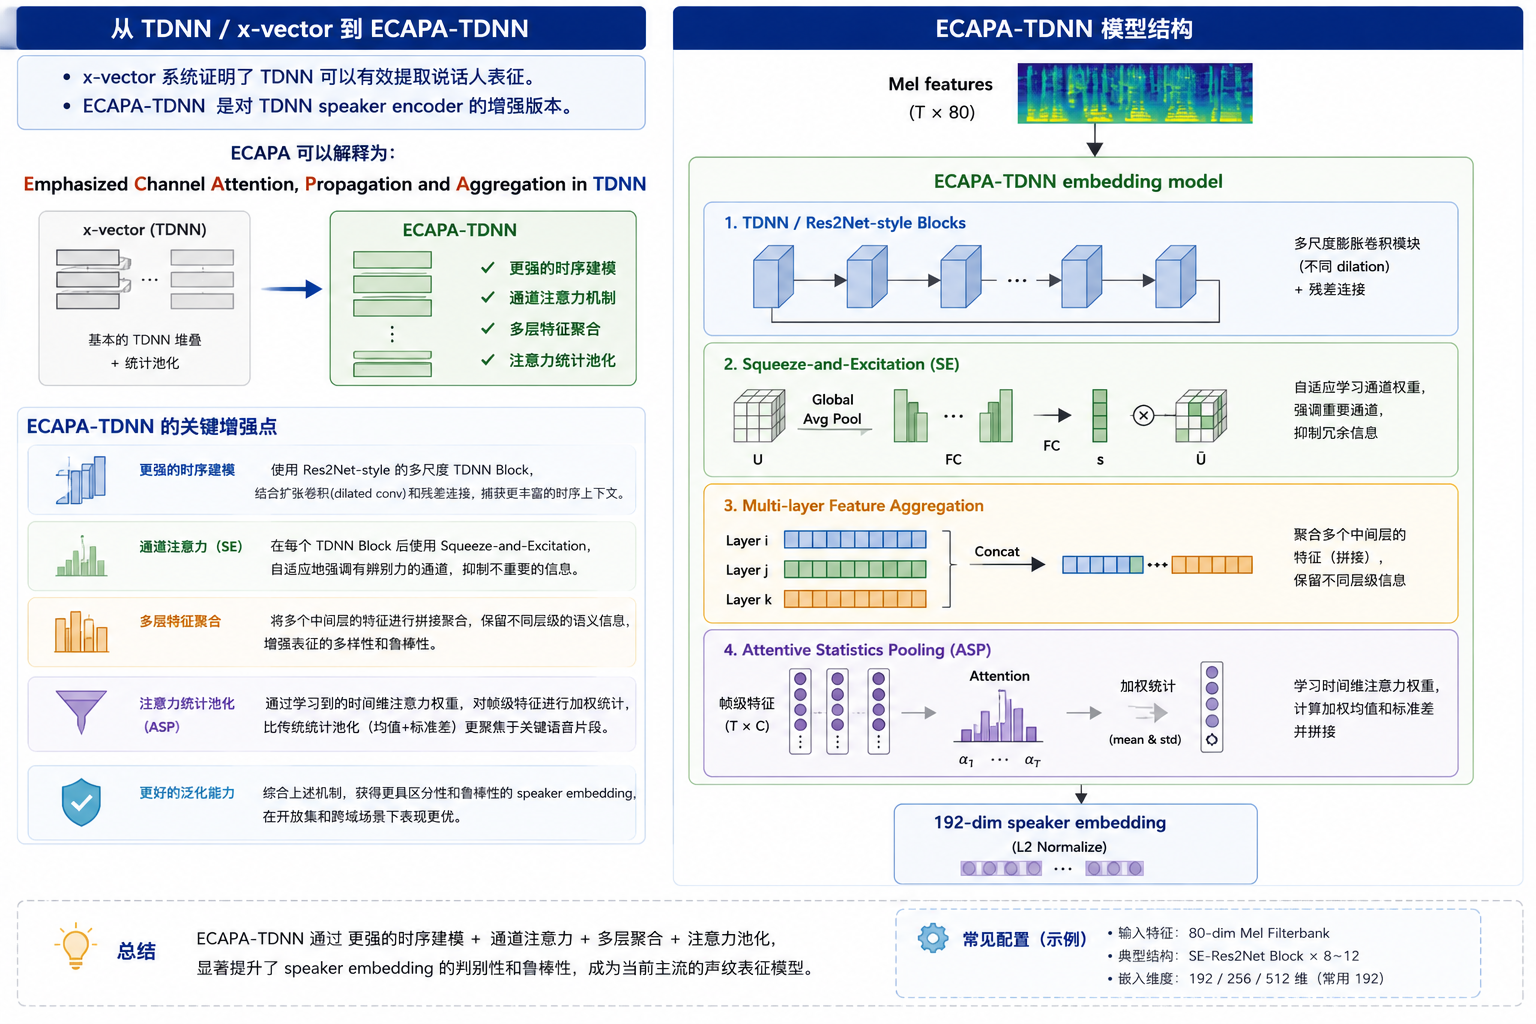
\includegraphics[width=0.8\textwidth]{ppt_ecapa_arch.png}
    \caption{ECAPA-TDNN 结构（引自课程课件）。}
    \label{fig:ecapa}
\end{figure}

嵌入经 L2 归一化后，两个向量的相似度用余弦相似度衡量，与角度间隔的训练目标一致。
对说话人 $s$ 的模板 $e_s$ 和测试嵌入 $\hat z_t$，
\begin{equation}
  \operatorname{score}(s,t)=\cos(e_s,\hat z_t)=e_s^\top \hat z_t .
\end{equation}
下游分两类任务。说话人验证判断一段语音是否属于某个指定说话人，把余弦分数与阈值 $\tau$ 比较得到判决。
随阈值定义错误接受率 FAR（把不同人判成同一人的比例）和错误拒绝率 FRR（把同一人误拒的比例），
两者相等处的错误率为等错误率 EER：
\begin{equation}
  \tau^\ast=\arg\min_{\tau}\bigl|\operatorname{FAR}(\tau)-\operatorname{FRR}(\tau)\bigr|,\qquad
  \operatorname{EER}\approx \tfrac12\bigl(\operatorname{FAR}(\tau^\ast)+\operatorname{FRR}(\tau^\ast)\bigr).
\end{equation}
说话人辨认判断一段语音属于哪个注册说话人，对每个说话人模板求分数取最大。
闭集直接取 $\hat s=\arg\max_s \operatorname{score}(s,t)$，开集要求最大分数超过阈值 $\tau_{id}$，否则判为 unknown。

\section{课程一：环境配置与说话人嵌入提取}
\subsection{模型加载与 checkpoint 结构}
从 HuggingFace 镜像下载 CN-Celeb ECAPA-TDNN checkpoint 到本地 \texttt{ckpt/spkrec-ecapa-cnceleb}，
用 \texttt{EncoderClassifier.from\_hparams} 加载，Windows 下采用 \texttt{LocalStrategy.NO\_LINK}
直接引用本地文件，避免符号链接权限问题。checkpoint 的 \texttt{hyperparams.yaml}（HyperPyYAML 格式）中的关键模块见表~\ref{tab:modules}。

\begin{table}[H]
  \centering
  \begin{tabularx}{\textwidth}{l X}
  \toprule
  模块 & 作用 \\
  \midrule
  \texttt{compute\_features} & 计算 Fbank（log-Mel）声学特征 \\
  \texttt{mean\_var\_norm} & 逐句（\texttt{norm\_type=sentence}）均值方差归一化 \\
  \texttt{embedding\_model} & ECAPA-TDNN 主体，输出 192 维嵌入 \\
  \texttt{classifier} & 训练阶段的说话人分类头，推理时不使用 \\
  \midrule
  \texttt{lin\_neurons}=192 & 嵌入维度 \\
  \texttt{out\_n\_neurons}=2793 & 训练集 CN-Celeb 的说话人类别数 \\
  \bottomrule
  \end{tabularx}
  \caption{ECAPA-TDNN checkpoint 的主要模块与超参。}
  \label{tab:modules}
\end{table}

\subsection{嵌入提取流程}
\texttt{encode\_batch} 依次执行：为一维 waveform 补上 batch 维、搬到设备并转 float、计算 Fbank 特征、
逐句均值方差归一化、送入 ECAPA-TDNN 得到嵌入。本实验对输出再做一次 L2 归一化，
使后续可以直接用点积算余弦相似度。对示例音频提取得到形状 \texttt{torch.Size([192])} 的嵌入，归一化后范数为 1。

\subsection{思考题}
\textbf{Q1（waveform 取值范围与幅度归一化）} \quad
\texttt{torchaudio.load()} 默认返回 \texttt{float32}、形状为 \texttt{[channel, time]} 的张量，取值在 $[-1,1]$；
\texttt{scipy.io.wavfile.read()} 读取 16-bit PCM 得到的是 \texttt{int16}，范围约 $\pm 3\times10^4$。
把未缩放的 int16 和缩放到 $[-1,1]$ 的 float 分别送入模型，两者幅度相差约三个数量级
（abs-max 为 1543 与 0.047），但得到的嵌入余弦相似度为 1.0000，与 \texttt{torchaudio.load} 的结果也一致。
原因是前端先取 log-Mel 再做逐句均值方差归一化，整体幅度的线性缩放在 log 域只是一个常数偏移，
会被句级归一化抵消，所以幅度不影响最终嵌入，需要保证的是波形形状而非绝对幅度。

\textbf{Q2（checkpoint 结构）} \quad
\texttt{modules} 含 \texttt{compute\_features}、\texttt{mean\_var\_norm}、\texttt{embedding\_model}、\texttt{classifier}
四部分（表~\ref{tab:modules}）。\texttt{lin\_neurons}=192 是嵌入维度，\texttt{out\_n\_neurons}=2793 是训练集
CN-Celeb 的说话人数。\texttt{encode\_batch} 只走到 \texttt{embedding\_model}，不经过 \texttt{classifier}；
分类头只在训练（\texttt{classify\_batch}）时把嵌入映射到 2793 个训练说话人上计算分类损失。

\textbf{Q3（嵌入维度是否可解释）} \quad
嵌入形状为 $[192]$。这 192 维并不逐维对应性别、口音、音高这类可解释因子，
它是端到端学到的分布式表示，因此比较时用整条向量，不看单独某一维。
但如果部分维度与性别、口音等属性相关，嵌入就可能间接泄露这些属性，对系统公平性和隐私有潜在影响（见课程二 Q2）。

\section{课程二：说话人嵌入空间与鲁棒性分析}
\subsection{干净嵌入的 t-SNE 可视化}
读取 \texttt{aishell\_mini} 的 metadata，对全部选中语句批量提取干净语音的嵌入并保存。
192 维无法直接可视化，用 t-SNE 投影到二维（\texttt{init="pca"}，\texttt{perplexity} 随样本数自适应），
用颜色区分说话人、用标记形状区分性别，结果见图~\ref{fig:tsne_clean}。
同一说话人的语句在二维平面上聚成清晰的簇，不同说话人相互分离，说明预训练嵌入在这个域上已经有很好的说话人可分性。

\begin{figure}[H]
    \centering
    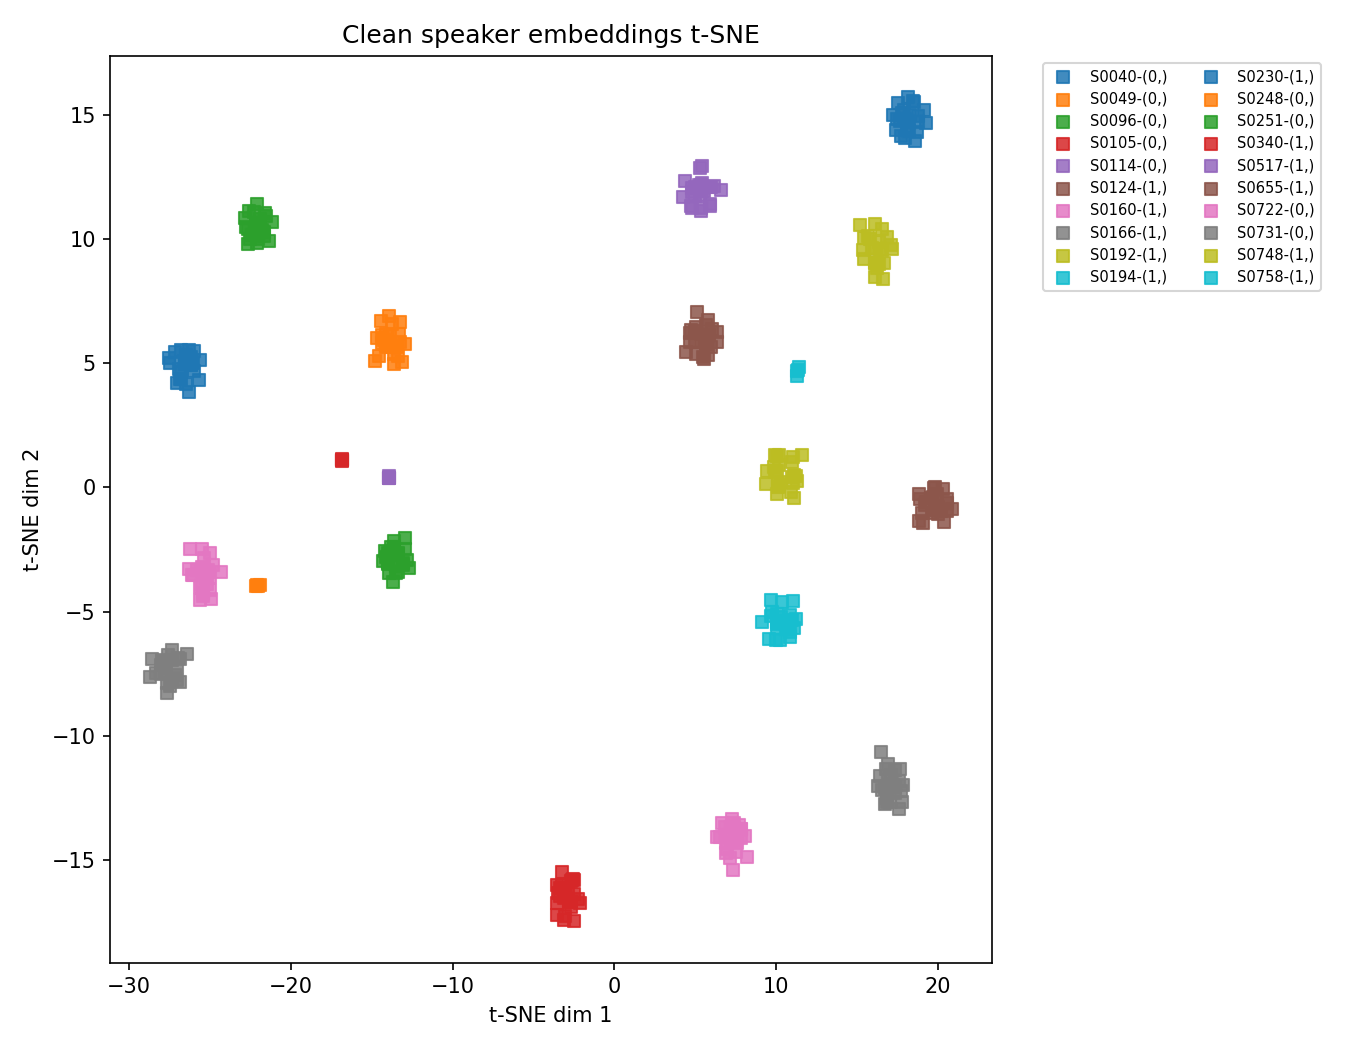
\includegraphics[width=0.7\textwidth]{res_tsne_clean.png}
    \caption{干净语音嵌入的 t-SNE。颜色表示说话人，标记形状表示性别，同一说话人聚簇明显。}
    \label{fig:tsne_clean}
\end{figure}

\subsection{三种扰动与嵌入漂移}
对同一批语音施加三种扰动：加性白噪声（按 SNR 10\,dB 缩放噪声叠加）、8k 电话信道模拟
（16k 到 8k 再回到 16k 的重采样，模拟带宽受限）、以及作为思考题 Q3 自选的变调
（pitch shift，$+4$ 半音，直接改变基频和共振峰位置）。把干净嵌入和扰动嵌入放进同一次 t-SNE 投影
（图~\ref{fig:tsne_joint}），并用 $1-\cos(\text{干净},\text{扰动})$ 度量逐句嵌入漂移，
按扰动类型统计见表~\ref{tab:drift}，箱线图见图~\ref{fig:drift}。

\begin{table}[H]
  \centering
  \begin{tabular}{lcc}
  \toprule
  扰动类型 & 平均余弦相似度 & 平均漂移 $1-\cos$ \\
  \midrule
  加噪 SNR 10\,dB & 0.704 & 0.296 \\
  8k 电话信道 & 0.514 & 0.486 \\
  变调 $+4$ 半音（自选） & 0.215 & 0.785 \\
  \bottomrule
  \end{tabular}
  \caption{三种扰动下的嵌入漂移，值越大表示嵌入偏离越多。}
  \label{tab:drift}
\end{table}

\begin{figure}[H]
\centering
\subfigure[干净与扰动嵌入的联合 t-SNE。]{
\begin{minipage}[t]{0.56\linewidth}
\centering
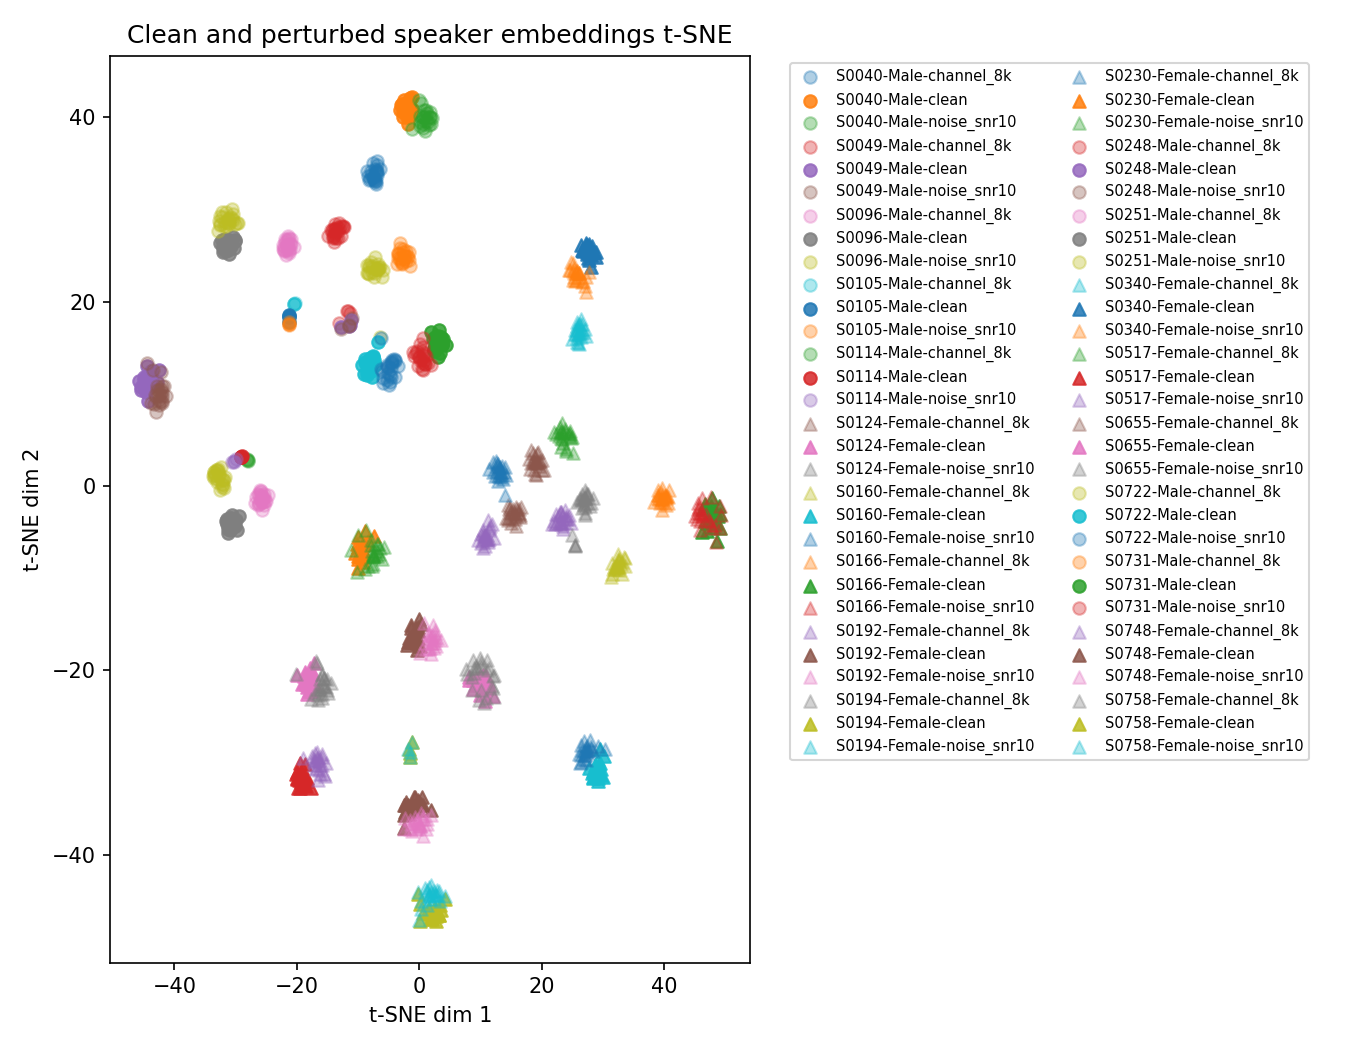
\includegraphics[width=\linewidth]{res_tsne_joint.png}
\label{fig:tsne_joint}
\end{minipage}}%
\subfigure[三种扰动的嵌入漂移箱线图。]{
\begin{minipage}[t]{0.42\linewidth}
\centering
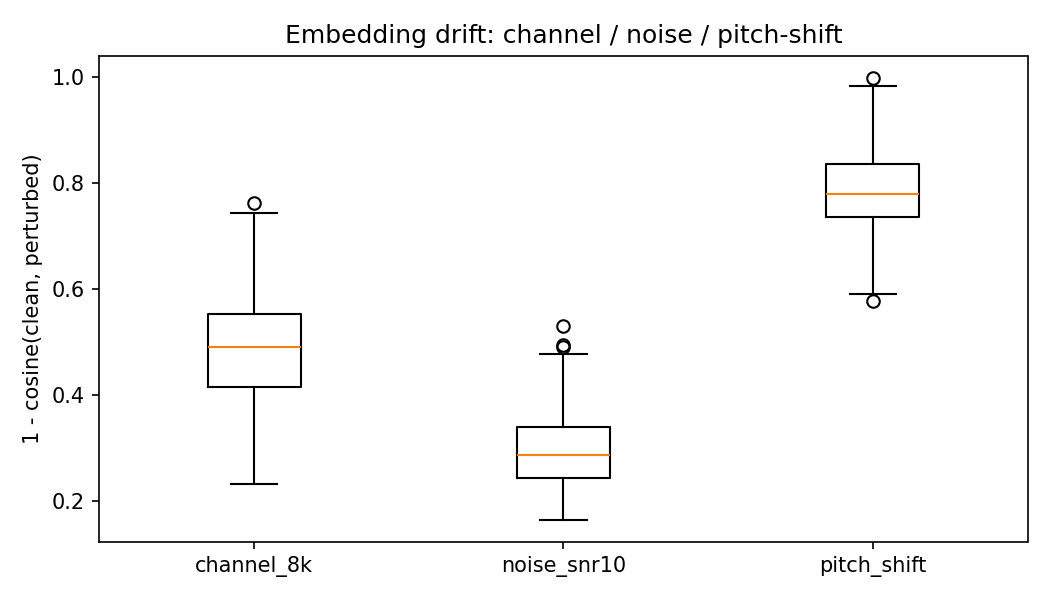
\includegraphics[width=\linewidth]{res_drift_boxplot.png}
\label{fig:drift}
\end{minipage}}
\caption{扰动对说话人嵌入的影响，变调漂移最大，信道次之，加噪最小。}
\label{fig:perturb}
\end{figure}

\subsection{思考题}
\textbf{Q1（为何联合做 t-SNE）} \quad
必须把干净嵌入和扰动嵌入放进同一次 t-SNE 拟合。t-SNE 每次拟合得到的坐标系是独立且非线性的，
两张分别拟合的图之间坐标不可比，直接比较点的位置没有意义。
只有共享同一次投影，图中干净点和它的扰动版本之间的相对位移才可读。

\textbf{Q2（性别聚类与其影响）} \quad
t-SNE 用标记形状表示性别，可以看到男女在空间中有一定的整体分区，说明嵌入除说话人身份外还带有性别信息。
这对识别系统有正反两方面影响：性别是一个粗粒度线索，有助于排除异性说话人，可能略微提升准确率；
但如果某一性别的样本偏少，该群体的错误率可能偏高，带来公平性问题；
同时嵌入可以被用来反推性别等敏感属性，超出身份比对本身，存在隐私风险。

\textbf{Q3（自选扰动是否改变说话人身份）} \quad
自选的变调（$+4$ 半音）平均漂移达 0.785，明显大于加噪的 0.296 和信道的 0.486。
加噪和信道主要叠加与说话人无关的噪声或损失高频，模型的句级归一化和噪声鲁棒性能抵消一部分；
变调则直接改变基频和共振峰，而这两者本身携带说话人身份信息，所以漂移最大，更接近改变了说话人本身。

\textbf{Q4（数据集 domain mismatch）} \quad
模型训练于 CN-Celeb，那里多是含噪、跨信道的采访和媒体语音；本实验推理于 AISHELL，是较干净的朗读语音。
录音条件和说话风格的差异构成 domain mismatch。不过迁移方向是从更难的域到更干净的域，
一般不会退化甚至更稳定，所以干净语音上的可分性和识别指标偏乐观；
如果换到更嘈杂的目标域，分布会明显变化，指标会下降。

\section{课程三：说话人验证与辨认}
\subsection{Enrollment 模板}
对每个注册说话人，取它若干条 enrollment 语句的 L2 归一化嵌入 $\hat z_{s,i}$，
先平均再做一次 L2 归一化得到说话人模板：
\begin{equation}
  e_s=\frac{\frac1K\sum_{i=1}^{K}\hat z_{s,i}}{\bigl\|\frac1K\sum_{i=1}^{K}\hat z_{s,i}\bigr\|_2}.
\end{equation}
平均相当于对随机的信道和内容扰动做平滑，得到更稳定的身份表示。

\subsection{说话人验证：EER 与阈值}
对每条 trial，用模板和测试嵌入的余弦相似度打分。在 dev 集上扫描 300 个候选阈值，
取 $|\text{FAR}-\text{FRR}|$ 最小处得 $\tau^\ast=0.4357$，此时 dev EER 接近 0，
同一说话人和不同说话人的分数分布几乎完全分开（图~\ref{fig:hist_dev}、图~\ref{fig:far_frr}）。
固定这个阈值迁移到 test 集评测（图~\ref{fig:hist_test}，表~\ref{tab:asv}）：
96 条 trial（正负样本各 48）中出现 2 次错误接受、0 次错误拒绝，即 test FAR 4.17\%、FRR 0、准确率 97.92\%。

\begin{table}[H]
  \centering
  \begin{tabular}{lccccc}
  \toprule
  数据集 & 阈值 $\tau$ & EER 或 FAR & FRR & 准确率 & 备注 \\
  \midrule
  dev  & 0.4357 & $\approx 0$ & $\approx 0$ & --- & 扫描确定 $\tau^\ast$ \\
  test & 0.4357 & 4.17\% & 0\% & 97.92\% & 96 条，2 次错误接受 \\
  \bottomrule
  \end{tabular}
  \caption{说话人验证结果，阈值在 dev 上确定后固定用于 test。}
  \label{tab:asv}
\end{table}

\begin{figure}[H]
\centering
\subfigure[dev 分数分布与阈值。]{
\begin{minipage}[t]{0.48\linewidth}
\centering
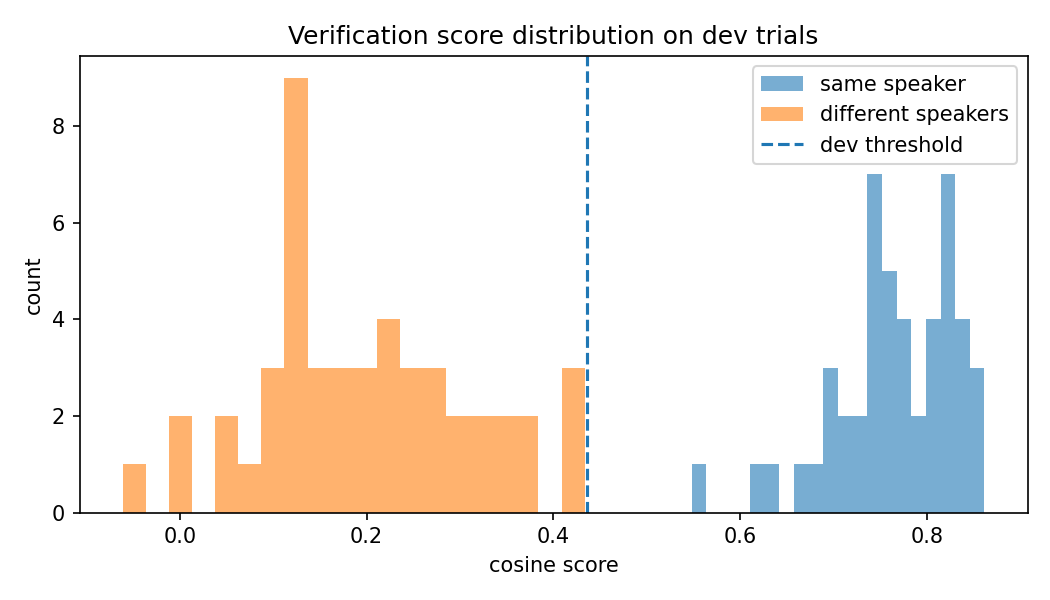
\includegraphics[width=\linewidth]{res_hist_dev.png}
\label{fig:hist_dev}
\end{minipage}}%
\subfigure[dev 上的 FAR 与 FRR 曲线。]{
\begin{minipage}[t]{0.48\linewidth}
\centering
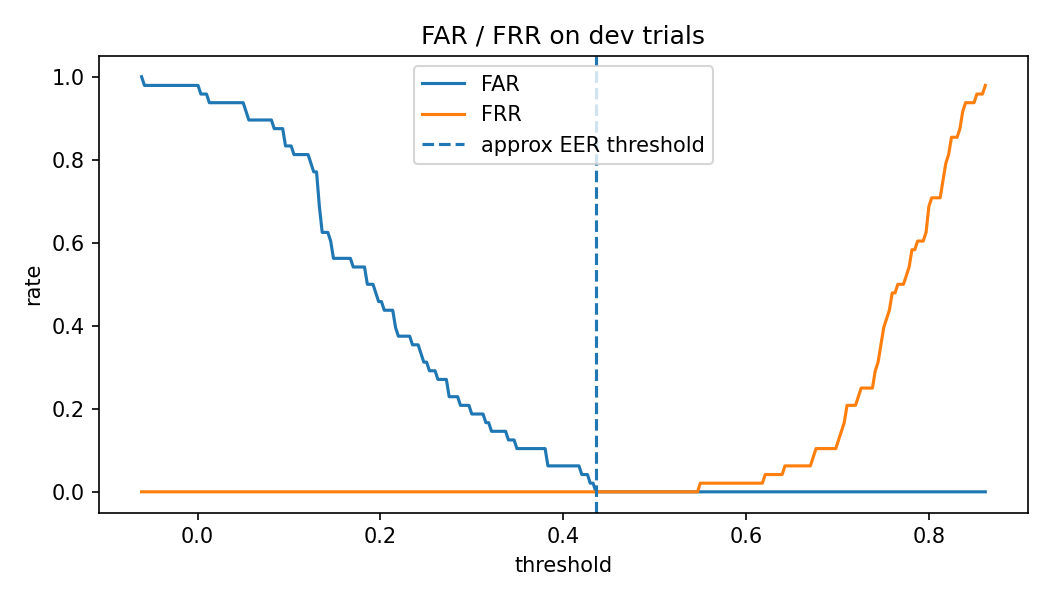
\includegraphics[width=\linewidth]{res_far_frr_dev.png}
\label{fig:far_frr}
\end{minipage}}
\caption{dev 集上的验证分数分布与 FAR、FRR 曲线，交点处即 $\tau^\ast$。}
\label{fig:dev_asv}
\end{figure}

\begin{figure}[H]
    \centering
    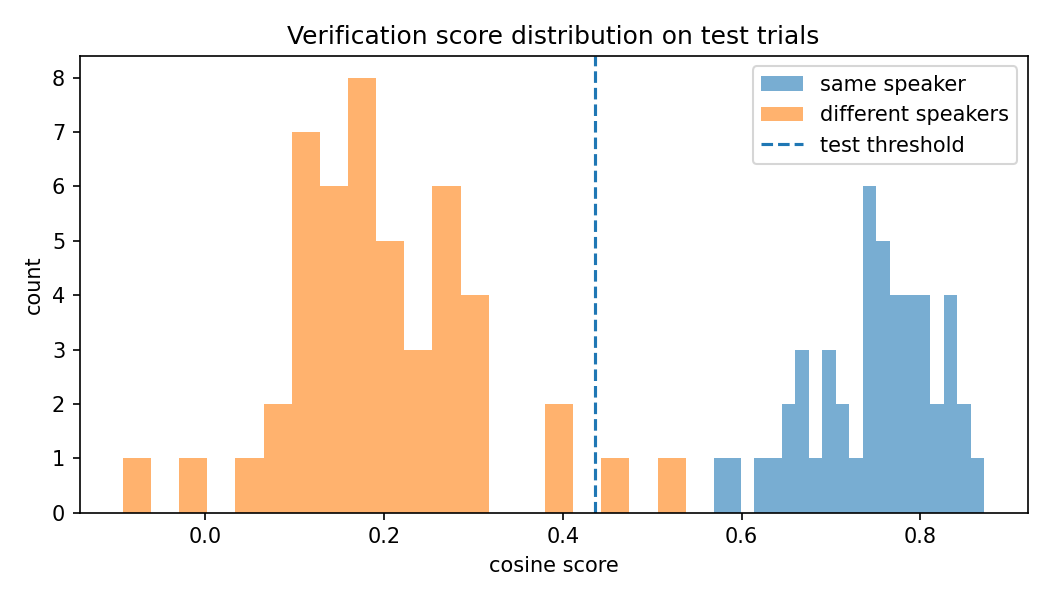
\includegraphics[width=0.6\textwidth]{res_hist_test.png}
    \caption{test 集验证分数分布，正负样本分离良好，仅少量负样本越过阈值。}
    \label{fig:hist_test}
\end{figure}

\subsection{说话人辨认：闭集与开集}
闭集辨认假定测试语音一定属于某个注册说话人，直接取分数最高者。64 条已知说话人语句的准确率为 100\%，
分数矩阵（图~\ref{fig:id_matrix}）呈明显的对角线主导，每条语句对其真实说话人模板的相似度都显著高于其他人。
开集辨认额外考虑未注册说话人，沿用 $\tau_{id}=\tau^\ast$，最高分低于阈值就判为 unknown。
16 条 unknown 语句中正确拒绝 11 条（拒识率 68.75\%），5 条被误判成某个注册说话人，
已知说话人的辨认准确率仍为 100\%。可见单一余弦阈值在开集下要在拒识率和已知识别率之间权衡。

\begin{figure}[H]
    \centering
    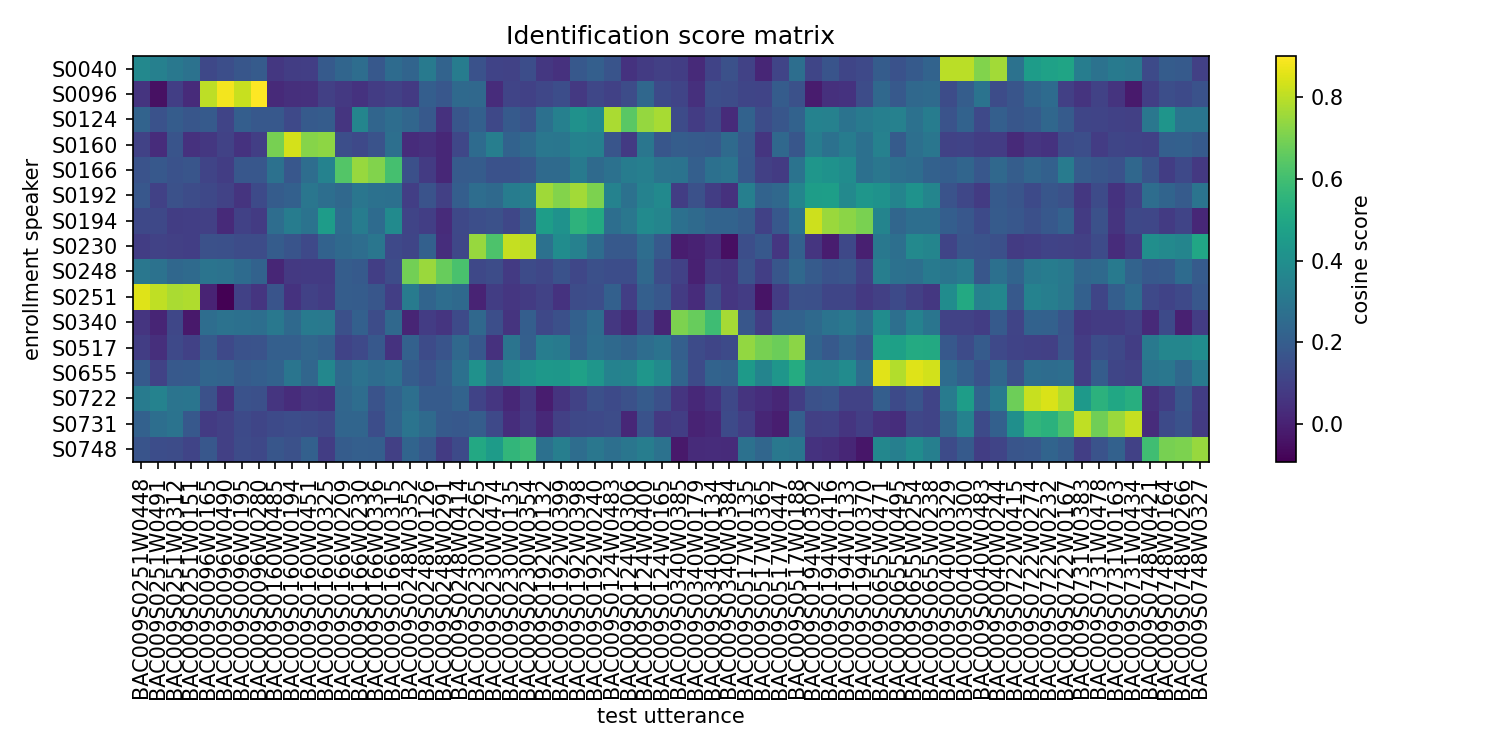
\includegraphics[width=0.85\textwidth]{res_id_matrix.png}
    \caption{闭集辨认的分数矩阵，行为注册说话人模板，列为测试语句。对角线主导，闭集准确率 100\%。}
    \label{fig:id_matrix}
\end{figure}

\subsection{加分项：嵌入之上的线性分类头}
加分项冻结 ECAPA 嵌入，在 \texttt{bonus\_train.csv} 的训练和验证划分上训练一个逻辑回归分类头，
做 16 类闭集说话人分类，训练和验证准确率都是 100\%。
这说明预训练嵌入已经高度线性可分，不微调主干、只加一个线性头就能得到很高的闭集准确率。

\subsection{思考题}
\textbf{Q1（单条 enrollment 的模板）} \quad
如果某说话人只有一条 enrollment，模板依然成立，就是这条 L2 归一化嵌入本身，
只是少了对信道和内容扰动的平滑，稳健性下降。多条平均能抑制单条语句的随机偏差，得到更接近说话人中心的表示。

\textbf{Q2（dev EER 为何这么小）} \quad
当前 \texttt{aishell\_mini} 说话人少、语音干净、trial 简单，同一和不同说话人的分数几乎完全分开，所以 dev EER 接近 0。
如果加入更难的负样本（比如同性别、口音相近的说话人）或改用完整 AISHELL1，EER 会明显上升，更接近真实水平。

\textbf{Q3（ASI 与 ASV 的区别）} \quad
说话人辨认回答语音是谁，是一对多，输出说话人编号或 unknown；说话人验证回答语音是不是某个人，是一对一，
输出相同或不同。两者都基于同一套说话人嵌入，区别在协议：验证的 trial 是注册人加测试语音加标签，用阈值判决；
辨认的 trial 是一条测试语音，和所有模板比较后取最大，开集再加阈值。

\textbf{Q4（为何用余弦相似度）} \quad
嵌入是固定维向量，L2 归一化后点积就是余弦相似度；模型训练用角度间隔损失，本来就在角度上区分说话人，
判决阶段用余弦和训练目标一致，度量最自然。要注意余弦分数只是相似度，并不直接等于概率，要做概率解释还需额外校准。

\textbf{Q5（阈值选择的权衡）} \quad
门禁安检类系统更怕错误接受（放进冒名者），应提高阈值来降低 FAR；
考勤签到类系统更怕错误拒绝（把真人挡在外面），应降低阈值来降低 FRR。
两类系统不应共用一个阈值，要按各自的错误代价分别标定。
实验中 $\tau^\ast-0.15$、$\tau^\ast$、$\tau^\ast+0.15$ 三档下 FAR 递减、FRR 递增，也印证了这一点。

\textbf{Q6（为何不在 test 上选阈值）} \quad
阈值是超参，应该在独立数据上确定。如果直接在 test 上扫阈值再报告该阈值下的 test 性能，等于用测试集调参，
会造成信息泄漏，指标偏乐观，不能反映真实泛化。实验里用 dev 选阈值得到的 test FAR 为 4.17\%，
而直接在 test 上取最优阈值得到的 EER 更低，两者的差距正说明了这个问题。

\textbf{Q7（为何模型能识别未见过的 AISHELL 说话人）} \quad
CN-Celeb checkpoint 的分类头固定输出 2793 个训练说话人之一，把一条 AISHELL 语句送进 \texttt{classify\_batch}
只会得到一个 CN-Celeb 类别编号，和真实的 AISHELL 说话人没有对应关系。
但嵌入网络学到的是通用的说话人表示，可以迁移到没见过的说话人。
本实验就是丢掉分类头、只用嵌入做模板比对，才能对 AISHELL 说话人做验证和辨认（闭集准确率 100\%）。
分类头服务于训练阶段的判别，能迁移的是嵌入网络。

\section{结论}
本实验用预训练 ECAPA-TDNN 作为说话人特征提取器，走通了从嵌入提取、可视化到验证与辨认的完整流程，主要结论如下：
\begin{enumerate}
  \item 说话人嵌入经句级归一化后对整体幅度不敏感，192 维向量以整体方向编码身份，干净语音上 t-SNE 聚簇清晰、线性可分。
  \item 三种扰动中变调引起的嵌入漂移最大（0.785），信道次之（0.486），加噪最小（0.296），
        因为变调改变了作为身份线索的基频和共振峰。
  \item 下游任务上，dev 扫描得 $\tau^\ast=0.4357$，test 验证准确率 97.92\%（FAR 4.17\%、FRR 0），
        闭集辨认 100\%，开集对 unknown 的拒识率 68.75\%，冻结嵌入上的线性分类头也达到 100\%。
  \item 分类头只服务于训练阶段，能迁移的是嵌入网络；阈值要在独立 dev 集上确定，并按错误代价按场景标定。
\end{enumerate}

\begin{thebibliography}{9}
\bibitem{ecapa} B. Desplanques, J. Thienpondt, K. Demuynck.
  \emph{ECAPA-TDNN: Emphasized Channel Attention, Propagation and Aggregation in TDNN Based Speaker Verification}.
  Interspeech, 2020. \url{https://arxiv.org/abs/2005.07143}
\bibitem{speechbrain} M. Ravanelli et al. \emph{SpeechBrain: A General-Purpose Speech Toolkit}.
  2021. \url{https://speechbrain.readthedocs.io}
\bibitem{arcface} J. Deng et al. \emph{ArcFace: Additive Angular Margin Loss for Deep Face Recognition}.
  CVPR, 2019. \url{https://arxiv.org/abs/1801.07698}
\end{thebibliography}

\end{document}
